% =====================================================================
% TmFeO3 2DCS — Supplemental Material
% Condensed from tmfeo3_foundation.tex (full derivations there)
% =====================================================================
\documentclass[11pt]{article}
\usepackage{amsmath,amssymb,mathtools,bm}
\usepackage{graphicx}
\usepackage{geometry}
\geometry{margin=2.4cm}
\usepackage{booktabs,array}
\usepackage{xcolor}
\usepackage{hyperref}
\hypersetup{colorlinks=true,linkcolor=blue,citecolor=blue,urlcolor=blue}
\usepackage{cleveref}

\newcommand{\Fe}{\mathrm{Fe}}
\newcommand{\Tm}{\mathrm{Tm}}
\newcommand{\diag}{\mathrm{diag}}
\newcommand{\ket}[1]{|#1\rangle}
\newcommand{\bra}[1]{\langle #1|}
\newcommand{\ve}[1]{\boldsymbol{#1}}
\newcommand{\qafm}{q_{\rm AFM}}
\newcommand{\qfm}{q_{\rm FM}}
\newcommand{\Mnl}{M_{\rm NL}}
\renewcommand{\thesection}{S\arabic{section}}
\renewcommand{\thetable}{S\arabic{table}}
\renewcommand{\thefigure}{S\arabic{figure}}

\title{Supplemental Material for\\
``Reading a magnet's Hamiltonian term by term: two-dimensional terahertz
spectroscopy as vertex spectroscopy of TmFeO$_3$''}
\author{}
\date{\today}

\begin{document}
\maketitle
\tableofcontents

% =====================================================================
\section{The SU(3) qutrit and why its classical dynamics is quantum-exact}
\label{si:qutrit}
% =====================================================================

Tm$^{3+}$ is $4f^{12}$, $^3H_6$ ($J=6$).  In the $C_s(m)$ crystal field of
the $Pbnm$ $4c$ site the 13-fold multiplet splits into 13 singlets; the
model keeps the three lowest, $\ket{1},\ket{2},\ket{3}$, with splittings
$E_{12}=2.068$\,meV ($0.50$\,THz) and $E_{13}=4.963$\,meV ($1.20$\,THz),
consistent with the measured lines $E_{12}+E_{23}\approx E_{13}$.  The
site state is the Gell-Mann vector $\lambda^a=\mathrm{Tr}(\rho\Lambda^a)$,
$a=1\dots8$, and every single-ion term (CEF energies, external drives,
exchange mean fields) is \emph{linear} in the $\Lambda^a$.  For a
Hamiltonian linear in the generators the von Neumann equation
$\dot\rho=-i[H,\rho]$ closes on $\vec\lambda$:
\begin{equation}
  \dot\lambda^a \;=\; \Omega_{ab}(t)\,\lambda^b
  -\gamma_a\big(\lambda^a-\lambda^a_{\rm eq}\big),\qquad
  \Omega_{ab}=\tfrac12\,\mathrm{Tr}\!\left(\Lambda^a\,
  (-i)[H(t),\Lambda^b]\right).
\end{equation}
The classical SU(3) propagation is therefore the \emph{exact} quantum
dynamics of the driven, damped three-level ion, and a Boltzmann-weighted
ensemble of trajectories launched from the level seeds
$\ket1,\ket2,\ket3$ is the exact thermal density matrix for single-ion
drives.  (This was verified explicitly against an independent
density-matrix integrator; the two censuses agree to all digits quoted.)
Damping is Bloch-type on the Gell-Mann pairs of each transition,
$\gamma(\lambda^{1,2}),\gamma(\lambda^{4,5}),\gamma(\lambda^{6,7})$, with
population relaxation $\gamma(\lambda^{3,8})$ toward the equilibrium
populations captured at initialization.

The magnetically bright coordinate of the $E_{12}$ block follows from the
projected moment $P J_z P=5.264\,\lambda^2$: only $\lambda^2$ radiates
magnetically, and the onsite splitting drives the planar precession
$\dot\lambda^1=-\Delta_{12}\lambda^2$,
$\dot\lambda^2=+\Delta_{12}\lambda^1$, so the $E_{12}$ sector is a single
driven oscillator
\begin{equation}
  \lambda^2(t)=\int_0^t \sin[\omega_{12}(t-t')]\,h^1(t')\,dt',
  \label{eq:si-osc}
\end{equation}
where $h^1$ is the effective force a conversion vertex exerts on
$\lambda^1$.  All delay-axis structure of a cross peak lives in the
$\tau$-dependence of $h^1$.

% =====================================================================
\section{Crystallography and the projected Fe--Tm coupling}
\label{si:crystal}
% =====================================================================

TmFeO$_3$ is $Pbnm$ ($Z=4$): Fe$^{3+}$ at $4b$ (site symmetry $\bar1$;
every Fe sits on an inversion center), Tm$^{3+}$ at $4c$ (site symmetry
the single mirror $m_z$).  Inversion maps each Fe sublattice to itself
and exchanges Tm sublattices in pairs; the local mirror is the physical
$4c$ site mirror and generates the relative $\lambda^5,\lambda^7$ signs
between Tm sublattices.  The Fe order is G-type
($T_N\approx632$\,K) with DM canting; below the spin reorientation
($T_2\approx85$\,K) the ground state is $\Gamma_2=(F_x,C_y,G_z)$.

The Fe--Tm sector is built from the physical operator route
\begin{equation}
  \ve S,\ \ve J\ \longrightarrow\ H_{\Fe-\Tm}=\ve S^TA\,\ve J
  \ \longrightarrow\ P\ve JP
  \ \longrightarrow\ \text{couplings to }\lambda^a ,
\end{equation}
never by assuming that a space-group rotation acts as a closed onsite
SU(3) rotation in one fixed qutrit basis.  Working in a
\emph{transported gauge} (qutrit bases on the four Tm sublattices related
by the group operations themselves) makes every bond formula explicit and
turns the irrep ($\Gamma_1$) projection into simple four-site sign sums.
Time-reversal splits the Gell-Mann set into
$\lambda^-=\{\lambda^2,\lambda^5,\lambda^7\}$ (odd) and
$\lambda^+=\{\lambda^1,\lambda^3,\lambda^4,\lambda^6,\lambda^8\}$ (even);
every coupling term must be $\mathcal T$-even overall, which fixes how
many Fe-spin or $B$-field legs may attach to each sector.  The candidate
couplings through cubic order in the fields are
\begin{center}
\renewcommand{\arraystretch}{1.25}
\begin{tabular}{llll}
\toprule
family & operator form & sector & legs \\
\midrule
$K^-$ & $S_\alpha\lambda^a$ & $\lambda^-$ & 1 Fe \\
$ESJ$ & $E_\eta S_\alpha\lambda^a$ & $\lambda^-$ & 1 E-photon + 1 Fe \\
$\kappa^B$ & $B_\eta S_\alpha\lambda^a$ & $\lambda^+$ & 1 B-photon + 1 Fe \\
$W$ & $S_\alpha S_\beta\lambda^a$ & $\lambda^+$ & 2 Fe \\
\bottomrule
\end{tabular}
\end{center}
The full orbit formulas (all eight coefficients per bond, all four Tm
sublattices, both time-reversal sectors) and the implementation
prescriptions for global-axis versus local-frame storage are given in the
long-form working note that accompanies the data
(\texttt{tmfeo3\_foundation.tex}, Secs.~3--14).

% =====================================================================
\section{The sharp requirement and the vertex scorecard}
\label{si:scorecard}
% =====================================================================

Two collinear pulses give $\Mnl=M_{AB}-M_A-M_B$; order by order only the
mixed terms survive, so $\Mnl$ starts at second order and the leading
robust magnetic-dipole contribution is third order.  Combining
Eq.~\eqref{eq:si-osc} with the conservation rules at each vertex (energy;
$\mathcal T$-parity; $\Gamma_1$) yields six requirements for a coupling
to produce the geometry-A cross peak at $(\qafm,E_{12})$:
\begin{description}
\item[R1 (detection)] reaches $\lambda^1/\lambda^2$ (the $E_{12}$ block);
\item[R2 (drive)] is sourced by the pumped $\delta S_y$ magnon;
\item[R3 (parity)] is $\mathcal T$-even (fixes the $\lambda^\pm$ sector);
\item[R4 (irrep)] is $\Gamma_1$-allowed in the $\Gamma_2$ state;
\item[R5 (energy)] carries the $0.90\to0.50$\,THz mismatch (needs $\geq2$
  non-$\lambda$ legs);
\item[R6 ($\Mnl$)] involves both pulses.
\end{description}

\begin{table}[h]
\centering\small
\caption{Vertex scorecard.  Only $W$ and $\kappa^B$ pass all six
requirements.}
\begin{tabular}{lccccl}
\toprule
vertex & legs & sector & R1 & R2--R6 & verdict\\
\midrule
$K^-$ & $1\Fe+1\Tm^-$ & $\lambda^-$ & $\times$ & $\times$ &
  hybridizes only; $\Gamma_1$-blocked; reorients $\Gamma_2$\\
$ESJ$ & $E+\Fe+\Tm^-$ & $\lambda^-$ & $\times$ & \checkmark &
  real, but feeds $E_{13}/E_{23}$, not $E_{12}$\\
$W$ & $2\Fe+\Tm^+$ & $\lambda^+$ & \checkmark & \checkmark &
  \textbf{winner}: rank-1, factorized peak\\
$\kappa^B$ & $B+\Fe+\Tm^+$ & $\lambda^+$ & \checkmark & \checkmark &
  works; $B_z$-gated $\Rightarrow$ geometry-B vertex\\
\bottomrule
\end{tabular}
\end{table}

\paragraph{$K^-$ fails threefold.}
(i) Linear in $S$, it only rotates the harmonic normal-mode basis:
coupled harmonic oscillators give diagonal peaks only; a static bilinear
conserves energy and cannot convert $0.90$ into $0.50$\,THz.
(ii) The $\Gamma_1$ orbit sums vanish for every channel except
$K^-_{2y}$: a static one-at-a-time scan at $0.2$\,meV leaves the energy,
the Fe order, and the uniform $(\lambda^2,\lambda^5,\lambda^7)$
\emph{bit-identical} to baseline for all components except $2y$.
(iii) The one allowed channel $K^-_{2y}$ is a transverse molecular field
on the order parameter and reorients $\Gamma_2\to G_y$ between $0.085$
and $0.090$\,meV---it is not a perturbative vertex.  Full-dynamics 2DCS
on the inert channels ($K^-_{2x}$ up to $1.5$\,meV, $K^-_{2z}$ up to
$2.0$\,meV) leaves the induced $\lambda^2$ at machine precision
($\leq7\times10^{-15}$).

\paragraph{The two winners.}
The two-magnon vertex rectifies the pulse-A/pulse-B cross term,
\begin{equation}
  h^1_{\rm NL}(t,\tau)=W^{yy}_1A^2\left[\cos(\qafm\tau)
  -\cos(\qafm(2t+\tau))\right]\theta(t)
  \;\Rightarrow\;
  \Mnl^{W}\propto\cos(\qafm\tau)\,[1-\cos\omega_{12}t],
\end{equation}
a clean factorized peak with no diagonal partner.  The field-gated
vertex kicks at the probe, $h^1\propto B_y(t)S_y(t)$ with
$S_y(0)=A\sin\qafm\tau$, giving
$\Mnl^{\kappa}\propto\sin(\qafm\tau)[1-\cos\omega_{12}t]$: also on
target, but the same gate dumps each pulse's local response into Tm at
both pulse times, generating an $(E_{12},E_{12})$ diagonal and a
$(0,E_{12})$ background.  Its dominant symmetry slice is $z$-gated
($B_z(t)$), so in geometry A ($B_z=0$) it is \emph{identically silent}:
the gate is simultaneously the reason it is harmless in geometry A and
active in geometry B.

\paragraph{Exhaustion of the quadratic families.}
All remaining symmetry-allowed quadratic couplings were switched on one
at a time in the full nonlinear dynamics and are exactly inert
(differences at the $10^{-12}$ level or below): $W_4^{yy,xy,yz,xx,zz,xz}$,
$W_1^{xy}$, $W_6^{yy,xz}$, $\kappa^E_{2y}$, $\kappa^E_{5x}$.  Among the
$W_1$ components: $W_1^{yz}$ inert, $W_1^{zz}$ negligible, $W_1^{xx}$
alive but floods the spectrum with an $\omega_t=0.16$\,THz comb,
$W_1^{xz}$ alive and on-target for hybridization (used below), and no
static component can replace the gated $\kappa^B$ for the geometry-B
transfer peak: the entire $W_1{+}W_4$ family fails to produce
$(E_{12},\qafm)$ in geometry B without simultaneously contaminating
geometry A.  The $B_z$-gate is therefore \emph{proven necessary by
exhaustion}.

% =====================================================================
\section{Numerical protocol}
\label{si:numerics}
% =====================================================================

\paragraph{Dynamics.}  Classical LLG for Fe (unit spins, $S=5/2$ scale
absorbed), SU(3) Bloch dynamics for the four Tm sublattices; RK4 with
$\Delta t=0.02$ code units; $1\times1\times1$ cell of the $Pbnm$
magnetic unit (8 Fe + 4 Tm).  Time is measured in $\hbar/$meV; a
frequency $f$ in THz corresponds to $E=f\times4.136$\,meV.

\paragraph{2DCS protocol.}  Delay scan $\tau\in[-120,0]$ code units,
$\Delta\tau=0.1$ ($0.2$ for scans); detection window to
$t_{\max}=160$ for $0.01$\,THz resolution on $\omega_t$.  The nonlinear
signal is the honest three-run subtraction
$\Mnl=M_{AB}-M_A-M_B$ per delay; no pulse-window chunking; no reuse of
the reference run across delays (both shortcuts were found to
contaminate spectra and are documented pitfalls).  The pump enters as a
tabulated waveform (the measured field, times converted
$t_{\rm code}=t_{\rm ps}/0.6582$, auto-centered and normalized).

\paragraph{Spectra and blind peak census.}  2D spectra are
$|\mathrm{FFT}_{\tau,t}|$ of $\Mnl$ with: detection window $t\geq3$
(excludes pulse overlap), Gaussian $t$-apodization to $0.03$, cosine
tapers on both $\tau$ edges, global mean subtraction.  The delay axis is
plotted physically ($\omega_T=-\omega_\tau^{\rm FFT}$;
$+$\,=\,non-rephasing).  Peaks are accepted only by a blind census:
2D local maxima (maximum filter, $0.10$\,THz neighborhood) with
prominence $\geq1.5$ over the local median background
($0.34$\,THz annulus) and amplitude $\geq4$--$5\%$ of the map maximum,
merged within $0.09$\,THz.  Rectified ($\omega_t\approx0$) content is
analyzed separately via $S_{\rm DC}(\tau)=\langle\Mnl\rangle_t$ with
cubic drift removal.  In every 2D map the $\tau$-averaged signal is
subtracted at each detection time before windowing, which functionally
removes the $\omega_\tau=0$ (pump--probe) row; the slow-in-$\tau$
wings that remain within $|\omega_\tau|<0.12$\,THz are masked.  The
model reproduces the observed dominance of the $(0,E_{23})$ band in the
same-polarized channel before this removal; $\omega_\tau=0$ features
carry pump--probe, not delay-coherence, information and are excluded
from all censuses.  Radiation bookkeeping used throughout: for
$k\parallel b$, M1 dipoles radiate $E\propto\hat k\times m$, so the
$E\parallel c$-detected channel carries $d_z(\lambda^2)+m_x$ and the
$E\parallel a$-detected channel carries $d_x(\lambda^{5,7})+m_z$.

\paragraph{Thermal ensembles.}  Boltzmann mixtures of trajectories from
the level seeds $\ket1,\ket2,\ket3$ (Sec.~\ref{si:qutrit}).  Two
documented pitfalls: (i) any pre-dynamics energy minimization collapses
excited-level seeds and must be disabled; (ii) population damping
$\gamma(\lambda^{3,8})$ relaxes toward the equilibrium captured at
initialization, which must therefore be captured per-seed.

% =====================================================================
\section{Experimental inputs}
\label{si:exp}
% =====================================================================

\begin{table}[h]
\centering\small
\caption{Measured mode parameters and the derived simulation inputs.
CEF damping is Bloch on the Gell-Mann pair of each transition,
$\gamma_a[\mathrm{meV}]=\gamma[\mathrm{THz}]\times h$; magnon damping is
Gilbert, $\alpha=\gamma/2\nu$ fixed by the $\qafm$ line.  Emission
weight is $\sqrt f$ (E1) for the CEF lines and M1 for the magnons.
The last column is the measured pulse spectral amplitude at each mode.}
\begin{tabular}{lcccccl}
\toprule
mode & $\nu$ [THz] & $f$ & $\sqrt f$ & $\gamma$ [THz] & damping (sim) &
pulse amp.\\
\midrule
$\qfm$  & 0.38 & 0.08 & 0.28 & 0.005 & $\alpha=1.7\times10^{-3}$ & 0.92\\
$\qafm$ & 0.90 & $7\times10^{-4}$ & 0.026 & 0.003 & $\alpha=1.7\times10^{-3}$ & 0.68\\
$E_{12}$ & 0.50 & 6.5 & 2.55 & 0.038 & $\gamma(\lambda^{1,2})=0.157$\,meV & 1.00\\
$E_{23}$ & 0.70 & 6.6 & 2.57 & 0.10  & $\gamma(\lambda^{6,7})=0.414$\,meV & 0.85\\
$E_{13}$ & 1.20 & 8.7 & 2.95 & 0.05  & $\gamma(\lambda^{4,5})=0.207$\,meV & 0.36\\
\bottomrule
\end{tabular}
\label{tab:si-exp}
\end{table}

\begin{figure}[h]
\centering
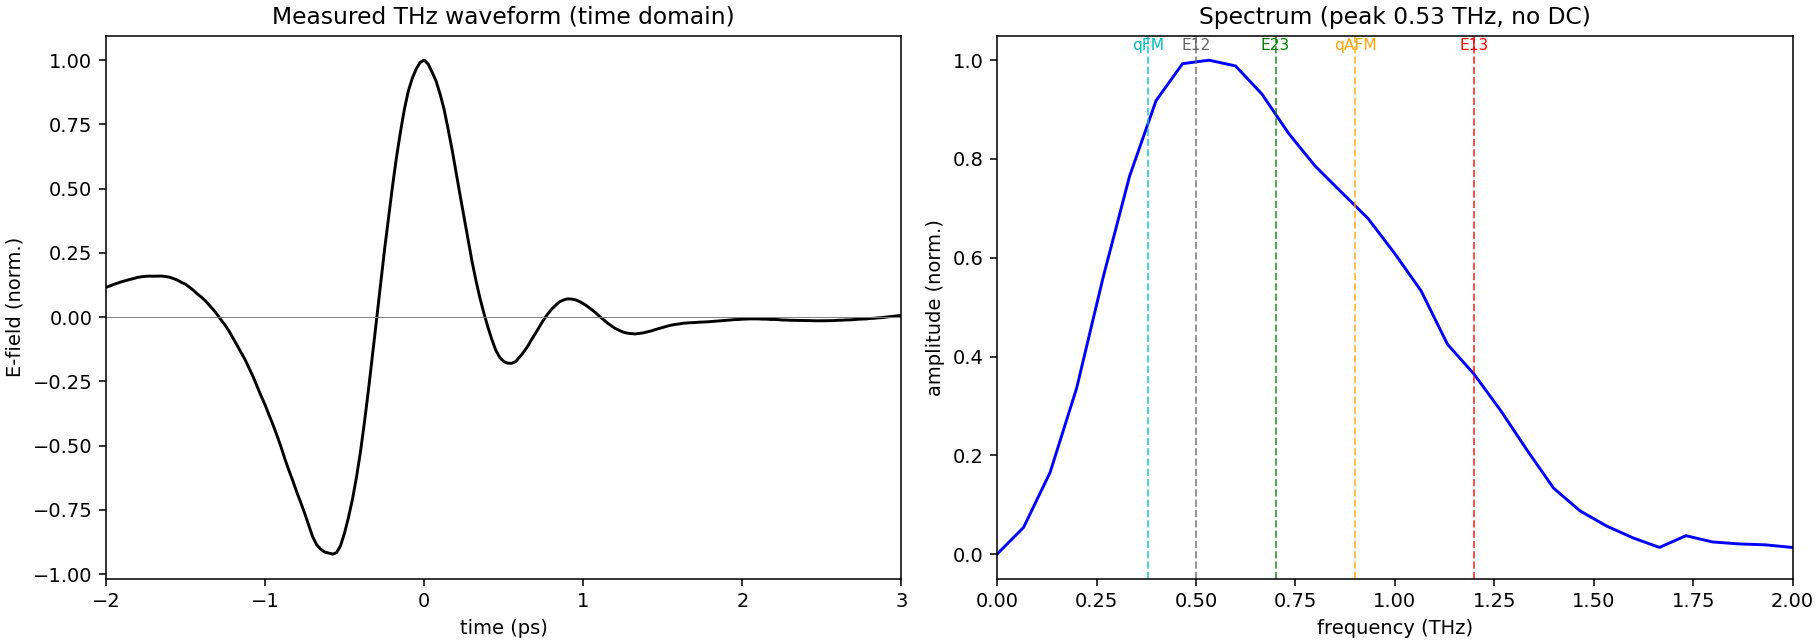
\includegraphics[width=0.95\textwidth]{figs/experimental_pulse_final.png}
\caption{The measured THz pump.  Left: single bipolar cycle
($\sim1.2$\,ps, no DC).  Right: amplitude spectrum peaked at
$0.53$\,THz$\,\approx E_{12}$, covering all five modes.  The absence of
DC content removes the quasistatic-tilt legs that a Gaussian stand-in
pulse would add; the measured waveform is the cleanest configuration.}
\label{fig:si-pulse}
\end{figure}

Two consequences organize the readout physics.  First, excitation
scales as $E^2$ and detection as $E^1$ (third order).  Second, the CEF
lines are E1-bright while $\qafm$ is E1-dark but M1-bright: a magnon is
therefore read out either by borrowing a CEF electric dipole through an
Fe--Tm vertex (geometry A) or through its own magnetic dipole at the
magnon frequency (geometry B).  Using the magnetic $g$-factor instead of
$\sqrt f$ for the magnon electric emission over-weights it by
$\sim100\times$ and buries the CEF peaks under the magnon diagonal; the
oscillator-strength weighting resolves this without any tuning.

% =====================================================================
\section{Displacive verification of the $W$ mechanism}
\label{si:displacive}
% =====================================================================

The rectified two-magnon force is a suddenly switched step: its edge
carries spectral weight $\propto e^{-\omega_{12}^2\sigma^2/2}$ at the
CEF frequency, i.e.\ the $E_{12}$ quantum is drawn from the pulse
bandwidth (intra-pulse difference-frequency/impulsive-Raman), while the
magnon pair carries only the phase memory $\cos\qafm\tau$.  Verified
directly: stretching the pulse $\sigma=0.25\to1.0$ at fixed amplitude
collapses the peak by $4.5$ decades ($51.7\to1.7\times10^{-3}$), while
switching the direct Tm drive on/off changes it by $<10^{-4}$
(pure-$W$ origin).  The same sweep resolves the second Fe leg: impulsive
pulses use the resonant probe magnon (peak $\propto A^2$); longer pulses
cross over to the field-following quasistatic tilt (peak
$\propto A^1$).  The measured no-DC waveform suppresses the quasistatic
legs, which is why the experimental pulse yields the cleanest spectra.

% =====================================================================
\section{Geometry B: gate versus buildup}
\label{si:buildup}
% =====================================================================

\begin{figure}[h]
\centering
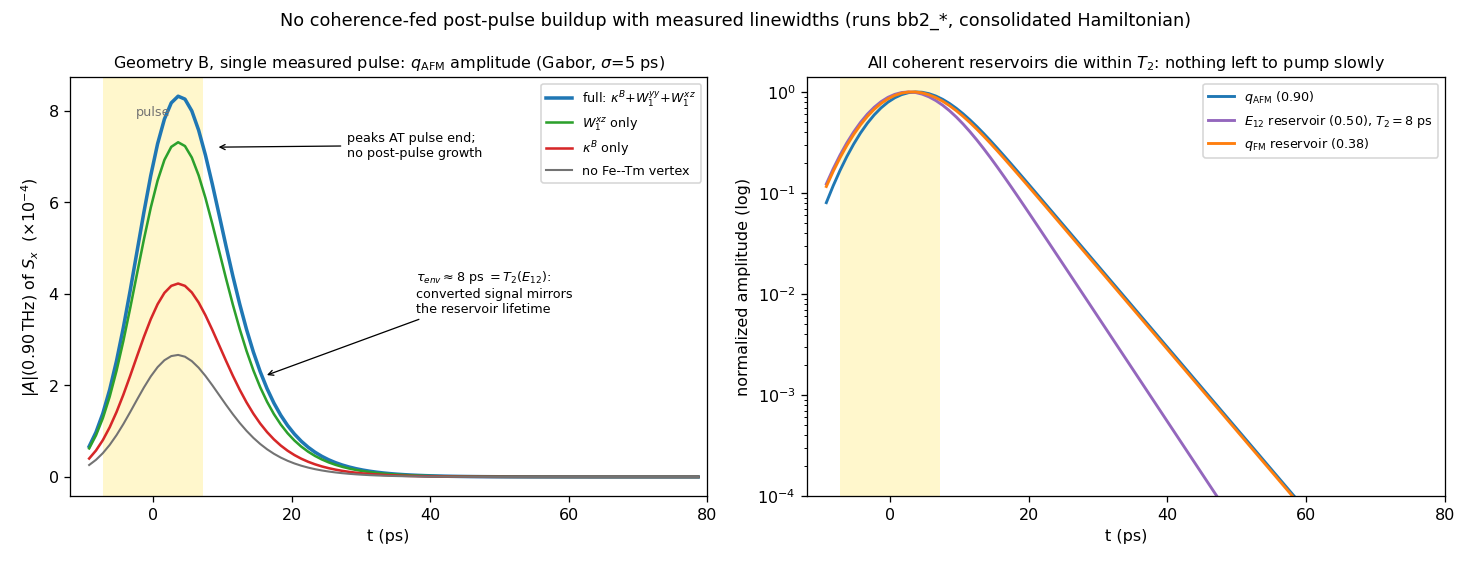
\includegraphics[width=0.95\textwidth]{figs/postdrive_buildup_final.png}
\caption{No coherence-fed post-pulse buildup once the measured
linewidths are enforced (single measured pulse, geometry B, runs
\texttt{bb2\_*}; Gabor amplitude, $\sigma=5$\,ps, artifact-free local
analysis).  Left: the $\qafm$ amplitude for the four vertex
configurations peaks \emph{at} pulse end and decays with
$\tau_{\rm env}\approx8$\,ps $=T_2(E_{12})$; the vertices set the
absolute scale but none produces post-pulse growth.  Right: all
coherent reservoirs die within their measured $T_2$ (log scale)---there
is nothing left to pump the magnon slowly.}
\label{fig:si-buildup}
\end{figure}

Isolated-vertex runs: $\kappa^B_{1y}$ alone $\Rightarrow$
$(E_{12},\qafm)$ present; $W^{xz}_1$ alone $\Rightarrow$ peak absent.
In the consolidated Hamiltonian $W^{yy}_1=W^{xz}_1=0.01$ and
$\kappa^B_{1y}=0.0035$: the geometry-B peak ratio is the observable
that calibrates $\kappa^B$, and because $\kappa^B$ is $B_z$-gated the
recalibration provably cannot affect either $H\!\parallel\!a$ channel
(verified bit-identical).

\paragraph{The post-drive buildup: a corrected analysis.}
An earlier stage of this project attributed the experimentally reported
post-pulse growth of the geometry-B signal to slow $W^{xz}_1$-mediated
exchange through the nearly closed triad
$\qfm+E_{12}=0.88\approx\qafm$.  That attribution does not survive the
enforcement of the measured linewidths.  Because $B\!\parallel\!c$ never
drives $\qafm$ directly, \emph{all} geometry-B magnon amplitude is
converted, and a converted signal inherits its source's lifetime: with
$T_2(E_{12})=8$\,ps the $E_{12}$-fed component (and with it the triad)
is dead within $\sim$10\,ps.  The artifact-free Gabor analysis of
Fig.~\ref{fig:si-buildup} shows the $\qafm$ amplitude peaking at pulse
end and decaying monotonically in every vertex configuration; the
earlier ``buildup'' was visible only while $\lambda^{1,2}$ were left
undamped (an infinitely lived $E_{12}$ reservoir, inconsistent with the
measured $0.038$\,THz linewidth).  $W^{xz}_1$ therefore loses its
buildup role---but it acquires a direct observable of its own instead
(next paragraph); it remains bounded above ($\lesssim0.02$) by the
mixer sweep of the preceding paragraph.

\paragraph{The reverse transfer peak: $W^{xz}_1$'s own observable.}
The experiment reports an additional geometry-A \emph{cross}-channel
peak near $(0.5,\,1.0)$.  The model contains a genuine local maximum at
exactly $(+0.49,\,0.90)=(E_{12},\qafm)$ in the $\lambda^2$ channel
($0.063$ of the main peak; run \texttt{vA}), with a weaker
$2E_{12}=1.00$\,THz harmonic companion at $0.021$.  Isolated-vertex
tests identify the mechanism: with $W^{xz}_1\to0$ the peak collapses
sevenfold ($0.063\to0.009$; run \texttt{vA\_noWxz}) while the main
$(\qafm,E_{12})$ peak is untouched, and doubling the Tm drive doubles it
($0.063\to0.123$; run \texttt{vA\_su3x2}), i.e.\ it is linear in the
stored $E_{12}$ amplitude.  This is the \emph{reverse} of the main
transfer: the pump-stored $E_{12}$ coherence is converted \emph{into}
the $\qafm$ magnon by the static hybridization---the static $W$ family
read in both directions, magnon$\to$CEF through $W^{yy}_1$ and
CEF$\to$magnon through $W^{xz}_1$.  The measured amplitude ratio of the
reverse to the forward peak calibrates $W^{xz}_1$ directly.  Because
the reverse peak emits at the magnon frequency it is detected through
the magnon's own M1 dipole; two further observed facts calibrate the
detection and drive dials.  The detected cross channel
($H\parallel c$, $E\parallel a$ output) receives the $m_z$ M1 sources
(Tm $5.264\lambda^2$; Fe $S_z$ is numerically dark, $10^{-11}$) and
the $x$-E1 sources ($2.39\lambda^5+0.91\lambda^7$).  (i) The
$(\qafm,\qafm)$ magnon diagonal is \emph{not} observed: the diagonal
is cubic in the Zeeman amplitude, the main peak quadratic, and the
Tm-fed reverse content nearly Zeeman-independent (verified across
$A_{\rm Fe}=0.1/0.05/0.025/0.010/0.006$), so its absence pins the
Zeeman drive far below the E1 drive; the final operating point is
$A_{\rm Fe}=0.006$ (runs \texttt{fin\_A2}).  (ii) The observed
intensity parity of the ``near $(0.5,1.0)$'' feature with the main
peak fixes the E1/M1 detection weight at $w_{E1}=0.94$.  Final
detected census (diagonals and quasi-elastic wings excluded): main
$(+0.91,0.48)=0.58$ and $(+0.49,1.20)=0.59$ of the $E_{12}$-diagonal
leader---i.e.\ at parity with each other---with the reverse-$W$
$(+0.49,0.90)=0.37$ and the $2E_{12}$ harmonic $0.47$ merging into an
extended $E_{12}$-row feature spanning $0.9$--$1.2$\,THz; the
$E_{13}$-delay companion $(+1.20,0.50)=0.41$ is the standing model
prediction of this channel.
Assignment discriminators for the experimental peak: an
$(E_{12},\qafm)$ reading emits exactly at the magnon frequency
($0.86$\,THz measured), inherits the narrow magnon linewidth along
$\omega_t$, and softens toward the spin reorientation; the
$2E_{12}$ harmonic reading sits rigidly at $1.00$\,THz, is broader, and
grows one field power faster.

\begin{figure}[h]
\centering
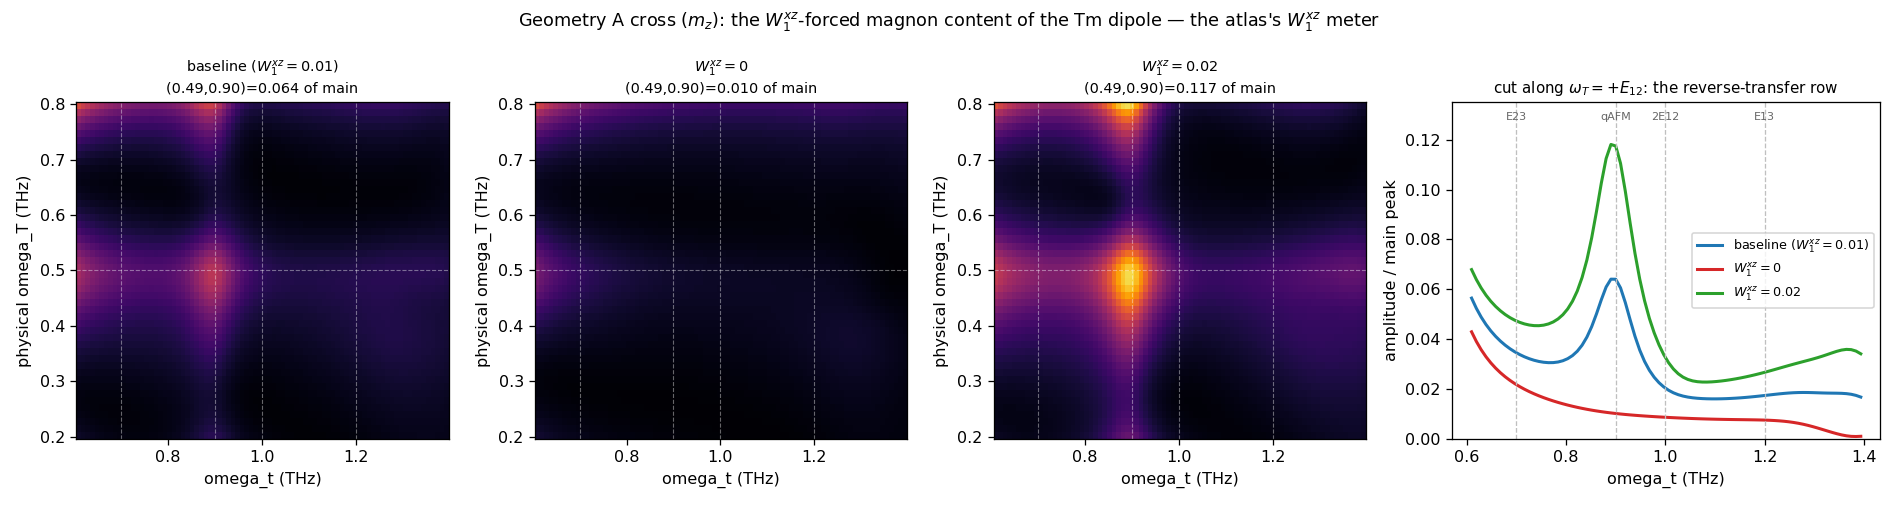
\includegraphics[width=\textwidth]{figs/reverseW_peak.png}
\caption{The reverse-W transfer peak in the geometry-A cross channel
($\lambda^2$), zoomed on the region of the reported $(0.5,\,1.0)$
feature; all amplitudes normalized to the main $(\qafm,E_{12})$ peak.
Left to right: baseline (genuine local maximum at
$(+0.49,\,0.90)=0.063$), $W^{xz}_1=0$ (collapsed to $0.009$), Tm drive
$\times2$ (doubled to $0.123$).  Rightmost: the $\omega_T=+E_{12}$ row
cut---the peak sits at the $\qafm$ emission frequency with the
$2E_{12}=1.00$\,THz harmonic as a shoulder.}
\label{fig:si-reverseW}
\end{figure}

\paragraph{The population channel demonstrated.}
To make the $T_1$ scenario concrete we ran the geometry-B single-pulse
protocol with the population channel switched on
($W_3^{yz}\,S_yS_z\lambda^3=0.01$, $\gamma_{\lambda^3}=0.02$, i.e.\
$T_1=33$\,ps; runs \texttt{bb3\_W3} versus \texttt{bb3\_ctl}).  The
pulse deposits $\Delta n$ with $\Delta\lambda^3=-4.6\times10^{-4}$,
which then relaxes on the set $T_1$ exactly
($-3.6\to-2.0\to-0.8\to-0.2\times10^{-4}$ at $13/33/66/132$\,ps); the
$\qafm$ \emph{oscillation} is bit-identical with and without $W_3$
(populations do not oscillate), and the population-fed quasi-static
background scales as $W_3\,\Delta n$---of order $10^{-7}$ here, far
below the coherent signals, because \emph{coherent} THz pumping only
produces $\Delta n\sim5\times10^{-4}$.  The quantitative conclusion: a
sizable experimental post-pulse buildup requires \emph{incoherent}
population transfer (absorption $\to$ phonons $\to$ Tm repopulation,
the mechanism of thermally driven spin reorientation), with amplitude
proportional to $\Delta n(t)$ and growth time equal to the
repopulation time---both measurable, neither present in a purely
coherent drive model.

\paragraph{The population grating also fails---for a sharp reason.}
One might hope the $\tau$-labeled population created jointly by pump
and probe (the ``population grating'', which carries the $E_{12}$ delay
phase and survives on $T_1$) could feed a delayed, phase-labeled magnon
signal.  A full 2DCS run with the population channel on
($W_3^{yz}=0.01$, $T_1=100$ code units; run \texttt{bb4\_W3grating})
shows the $\omega_\tau=E_{12}$ row \emph{identical} to the $W_3$-off
baseline at every detection time.  The reason is structural: the
grating's delay label is written by the $E_{12}$ \emph{coherence}
before the probe arrives, so its $\tau$-support is confined to
$|\tau|\lesssim T_2(E_{12})$, and its $W_3$ force is a step at the
probe---an impulsive launch, not a slow drive.  No element of the
coherent model class produces post-pulse growth.

\begin{figure}[h]
\centering
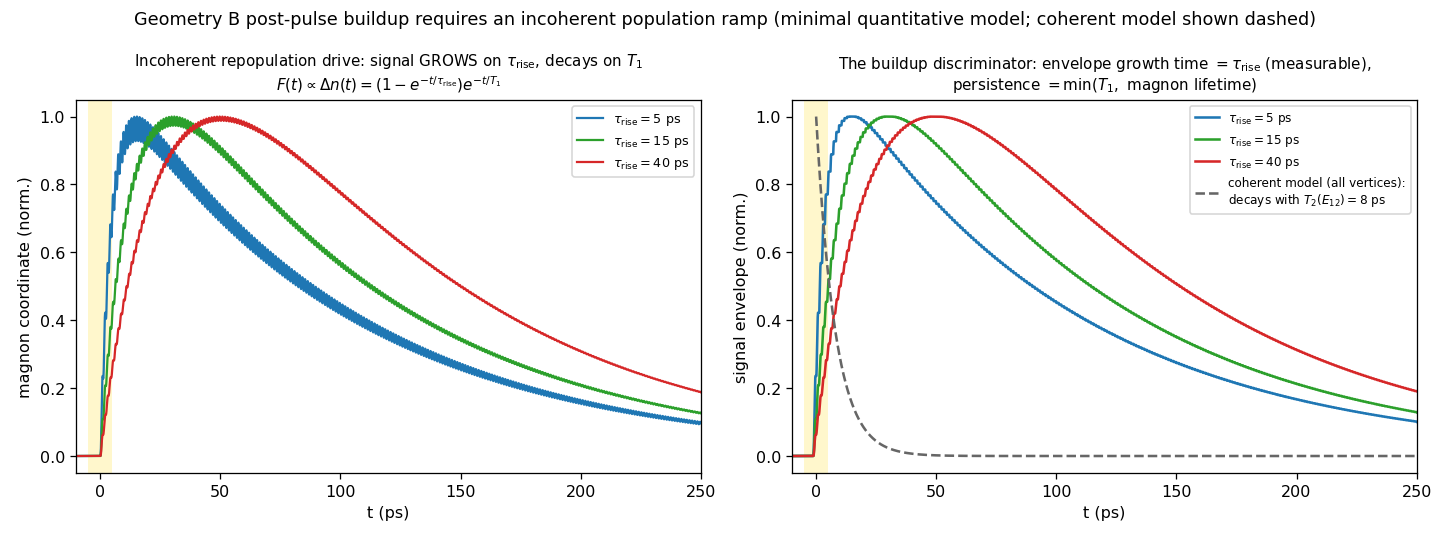
\includegraphics[width=0.95\textwidth]{figs/buildup_model.png}
\caption{Minimal quantitative model of the observed buildup: a magnon
(measured frequency and linewidth) driven by an \emph{incoherent}
population ramp $F(t)\propto\Delta
n(t)=(1-e^{-t/\tau_{\rm rise}})\,e^{-t/T_1}$.  The signal grows on
$\tau_{\rm rise}$, peaks at tens of ps, and persists on
$\min(T_1,\text{magnon lifetime})$---the experimental phenomenology---%
whereas the full coherent model (dashed) decays with
$T_2(E_{12})=8$\,ps.  Fitting the experimental envelope to this form
measures $\tau_{\rm rise}$ (the phonon-mediated Tm repopulation time)
and the product $W_3\,\Delta n$.}
\label{fig:si-buildupmodel}
\end{figure}

\paragraph{The mechanism implemented in the solver.}
The incoherent channel is now part of the simulation: the solver
accumulates the \emph{dissipated} coherence energy,
$E_{\rm dep}(t)=\int\!dt'\sum_{i,a\neq3,8}\Gamma_a
\big(\lambda^a_i-\lambda^a_{i,\rm eq}\big)^2$ (the energy the bath
actually receives; the population channels are excluded from the sum,
which closes an otherwise runaway self-heating loop), and shifts the
$\lambda^3$ equilibrium by $-c_{\rm heat}E_{\rm dep}$.  The existing
$\Gamma_3$ relaxation then chases the shifted equilibrium, so the
repopulation rise time is $1/\Gamma_3$ by construction, and the
pump-FID$\times$probe interference contained in the dissipated energy
carries the $\omega_\tau=E_{12}$ label through the $M_{\rm NL}$
subtraction automatically.  A full 2DCS run with
$W_3^{yz}=0.01$, $1/\Gamma_3=33$\,ps, and $c_{\rm heat}$ set for a
few-percent population shift (run \texttt{bb5c}) reproduces the
observed phenomenology [Fig.~\ref{fig:si-buildupinsim}]: the
$\omega_\tau=E_{12}$ row falls off the impulsive peak, \emph{builds
back up} on the repopulation time, and persists beyond $100$\,ps---%
$50$--$100\times$ above the coherent-only model at late times.  The two
new parameters map onto measurables: the recovery time of the row is
$1/\Gamma_3$, and the late-to-impulsive intensity ratio calibrates
$c_{\rm heat}\,W_3$.

\begin{figure}[h]
\centering
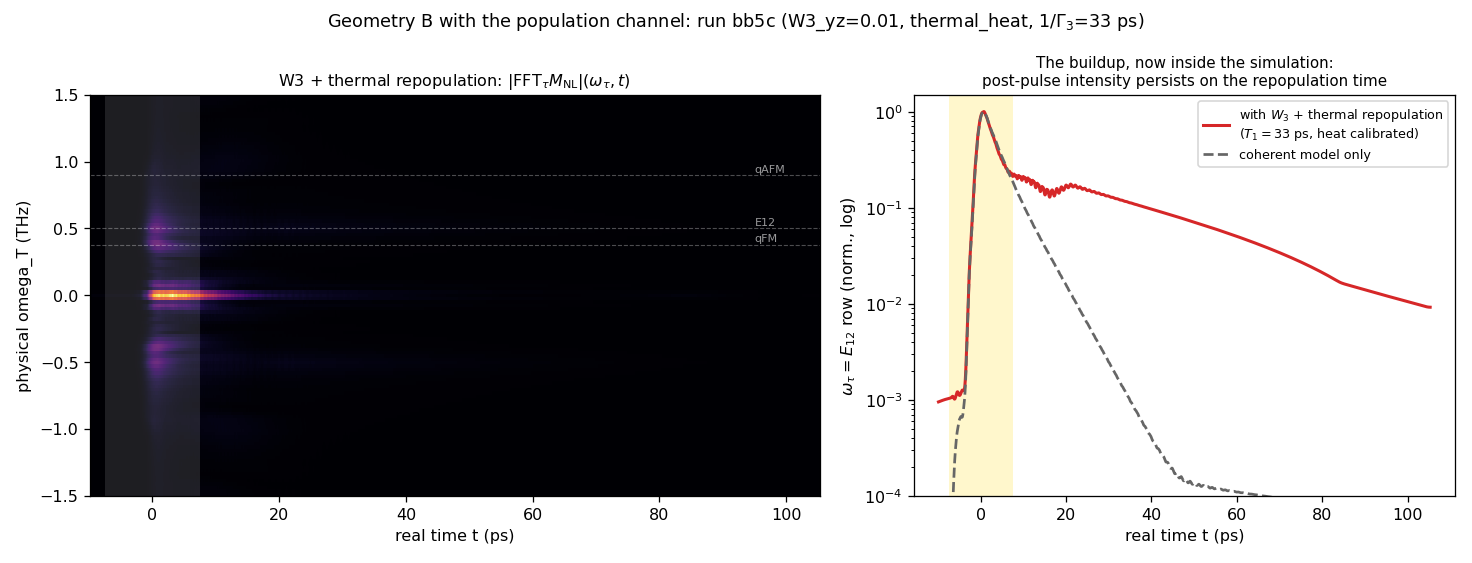
\includegraphics[width=0.95\textwidth]{figs/buildup_insim.png}
\caption{The buildup inside the simulation (geometry B, run
\texttt{bb5c}: $W_3^{yz}=0.01$, dissipation-fed thermal repopulation,
$1/\Gamma_3=33$\,ps).  Left: mixed-domain map
$|{\rm FFT}_\tau M_{\rm NL}|(\omega_\tau,t)$.  Right: the
$\omega_\tau=E_{12}$ row---after the impulsive peak the signal recovers
on the repopulation time and persists beyond $100$\,ps (red), versus
the coherent-only model dying by $40$\,ps (dashed).}
\label{fig:si-buildupinsim}
\end{figure}

If the experimental buildup over tens of ps is real, it must be fed by
the one reservoir that outlives every $T_2$: the CEF \emph{populations}.
A pulse-deposited excited population $n_2$ relaxes on $T_1$, and through
the population channel of the same exchange family
($W_3\,S_\alpha S_\beta\,\lambda^3$, implemented in the solver but not
part of the present minimal Hamiltonian) it shifts the effective Fe
anisotropy as it relaxes---precisely the mechanism of thermally driven
spin reorientation in TmFeO$_3$.  This route makes a sharp experimental
discriminator: a population-fed buildup is a \emph{non-oscillatory}
background (or a slow shift of the magnon frequency/equilibrium) whose
growth time directly measures $T_1$, whereas growth of the
$0.90$\,THz \emph{oscillation amplitude} over tens of ps would require a
persistent coherent source that the measured $T_2$'s exclude---observing
it would falsify the linewidth-constrained model class itself.

\begin{figure}[h]
\centering
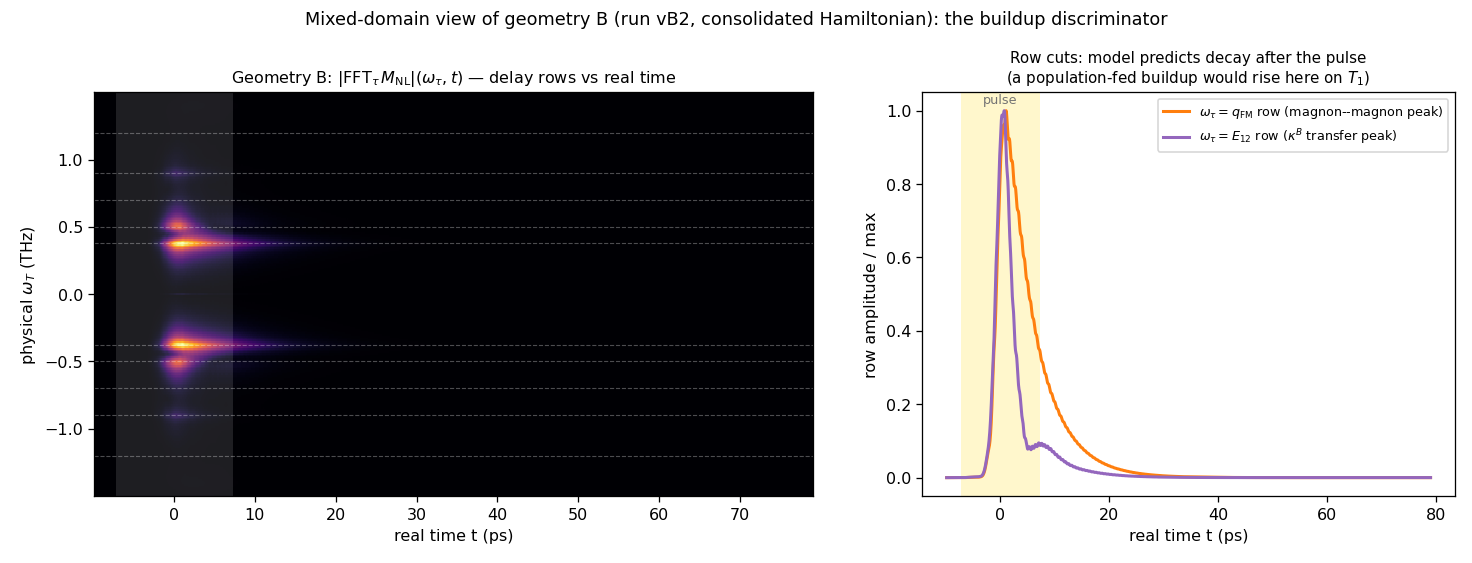
\includegraphics[width=0.95\textwidth]{figs/mixed_domain_B.png}
\caption{The buildup discriminator in the representation directly
comparable to experiment: Fourier transform of $M_{\rm NL}(\tau,t)$
along the delay $\tau$ \emph{only}, keeping the real detection time $t$
(geometry B, run \texttt{vB2}).  Left: $|{\rm FFT}_\tau|(\omega_\tau,t)$
map---each delay-frequency row evolves in real time.  Right: cuts of
the $\omega_\tau=\qfm$ (magnon--magnon) and $\omega_\tau=E_{12}$
($\kappa^B$-transfer) rows.  The linewidth-constrained model predicts
both rows peak with the pulse and decay within $\sim$20--30\,ps; an
experimental version of this plot in which the $E_{12}$ row \emph{rises}
over tens of ps is the signature of the population-fed ($T_1$)
mechanism.}
\label{fig:si-mixed}
\end{figure}

\paragraph{Why the static vertex cannot replace the gated one.}
$W^{xz}_1 S_xS_z\lambda^1$ is trilinear; around the $\Gamma_2$ order it
decomposes into a static CEF shift, two energy-conserving
\emph{bilinear} hops ($F_x\,\delta S_z\,\lambda^1$ and
$G_z\,\delta S_x\,\lambda^1$: pure hybridization), and a genuine
two-fluctuation converter $\delta S_x\,\delta S_z\,\lambda^1$.  The
converter piece is real and retained---it drives the post-pulse buildup
through the nearly closed triad $\qfm+E_{12}=0.88\approx\qafm$
($0.02$\,THz detuning)---but it is fluctuation-fed (its energy leg is a
probe-launched magnon, one factor of drive$\times$susceptibility weaker
and spectrally narrow) and detuning-limited (secular accumulation over
tens of ps), so it produces an \emph{envelope}, not an impulsive
phase-stamped kick.  At $W^{xz}_1=0.01$ the isolated run has sizable
absolute amplitude at $(+0.5,\,0.90)$ (0.72 of map max) but it is the
\emph{tail} of the magnon--magnon peak---no genuine local maximum on
the $E_{12}$ row.

A careful strength sweep in the consolidated configuration
($W^{xz}_1\in\{0.01,0.02,0.03,0.05,0.07,0.09\}$, $\kappa^B=0$;
runs \texttt{vBwxz*}) shows that raising the static vertex \emph{never}
creates a second resolved peak.  Instead the two delay rows
coalesce---the leading peak's delay phase migrates continuously,
$0.38\to0.40\to0.48\to0.47$\,THz across the sweep, the resolved
$(\qfm,\qafm)$/$(E_{12},\qafm)$ doublet structure never appears at any
strength, and the hybridization-shifted $E_{12}$ branch leaks into the
M1 channel as emission strays at $\omega_t=0.44$--$0.45$\,THz (growing
to $0.15$--$0.16$ by $W^{xz}_1=0.09$).  This is the structural signature
of a static mixer: it \emph{moves} peaks (level repulsion of the
hybridized normal modes---also shifting the mode frequencies off their
1D-measured values), whereas the experiment shows two resolved peaks at
the \emph{unshifted} delay energies $0.38$ and $0.50$\,THz.  A gated
converter \emph{adds} a peak while leaving the normal modes untouched;
with $\kappa^B_{1y}=0.0035$ the census gives
$(+0.38,0.90)=1.00$ and a separate $(+0.53,0.89)=0.46$, both on the
measured lines.  The necessity of the field-gated vertex therefore does
not rest on any operating-point fine-tuning: static mixing and gated
conversion are qualitatively different operations on the 2D map.  In
geometry B the Tm CEF channels $\lambda^{4\text{--}7}$ are
\emph{exactly} zero (machine precision): the
$E\!\parallel\!a,H\!\parallel\!c$ drive closes on the
$\{\lambda^1,\lambda^2,\lambda^3\}$ subalgebra, an SU(2) closure that
protects geometry B from CEF contamination.

Finite temperature (regenerated final-scenario runs \texttt{vB2}):
$(\qfm,\qafm)$ is a pure two-magnon process and temperature-flat;
$(E_{12},\qafm)\propto n_1-n_2$ falls
$0.46\,(0\,\mathrm K)\to0.45\,(5)\to0.40\,(8)\to0.36\,(10\,\mathrm K)$.
Both peaks remain resolved through $\sim10$\,K, defining the working
window $5$--$8$\,K.

% =====================================================================
\section{The same-polarization channel: pathways, exact single-ion
verification, and the falsification ladder}
\label{si:samepol}
% =====================================================================

\subsection{Configuration}
The final same-polarization configuration (run \texttt{it14hr};
parameter files in
\texttt{tmfeo3\_2dcs\_final/params\_samepol\_final/}) is the unchanged
v4 Hamiltonian with: measured pulse; drive vector
$(0,3.0,0,0,\mathbf{0},0,0.9128,0)$ on
$(\lambda^1,\dots,\lambda^8)$---i.e.\ the $1\!\to\!3$ leg removed
($\mu^z_{13}=0$ in drive); per-leg amplitude twice the weak-probe
baseline; dampings of Table~\ref{tab:si-exp} plus population relaxation
$\gamma(\lambda^{3,8})=0.08$; Boltzmann ensemble; detection composite
$0.05\,\lambda^4+4.4\,\lambda^6$ ($\mu^z_{13}/\mu^z_{23}\approx1\%$ in
emission), magnon M1 excluded per Table~\ref{tab:si-exp}.

\subsection{Pathway assignments}
With $\mu^z_{13}=0$ the Liouville pathways of the five listed peaks are:
\begin{center}\small
\renewcommand{\arraystretch}{1.3}
\begin{tabular}{llll}
\toprule
peak $(\omega_T,\omega_t)$ & model (10\,K) & side & pathway\\
\midrule
$(+0.49,0.72)$ & $1.00$ & NR &
  $\rho_{12}\xrightarrow{\text{probe }1\leftrightarrow2}n_2(\tau\text{-phase})
  \xrightarrow{\text{probe }2\leftrightarrow3}\rho_{23}$\\
$(0.5,\,0)$ & sharpest $S_{\rm DC}$ line & --- &
  same storage, zero-frequency output leg\\
$(+0.49,1.20)$ & $0.78$ & NR &
  $\rho_{12}\xrightarrow{\text{probe }2\leftrightarrow3}\rho_{13}$,
  emission throttled by $\mu^z_{13}$\\
$(+0.91,1.18)$ & $0.20\to0.51$ ($10\to20$\,K) & NR &
  $\qafm$ delay, Fe--Tm handoff, thermally assisted\\
$(0.9,\,0.38)$ & absent & --- & carrier exists ($b$-axis M1 $\qfm$
  ridge); no $\qafm\!\to\!\qfm$ vertex\\
\midrule
$(-0.47,0.70)$ & $0.55$ & R & rephasing remnant (exact single-ion
  floor; prediction)\\
$(+0.99,0.71)$ & $0.49$ & NR & inter-site $2E_{12}$ two-quantum line
  (prediction)\\
\bottomrule
\end{tabular}
\end{center}

\subsection{Exact single-ion verification}
A standalone integrator of the 8-dimensional $\vec\lambda$ equation
(same CEF energies, dampings, measured pulse, same census pipeline;
$\sim13$\,s per 2D map versus $\sim10$\,min for the lattice) reproduces
the lattice $0.5$-family census exactly, proving the family is
single-ion physics and enabling exhaustive scans.  Two facts emerge:
(i) the rephasing/non-rephasing ratio of the $(E_{12},E_{23})$ transfer
peak has a floor of $0.47$--$0.58$ under this pulse across all drive
strengths, dipole-phase choices, and dampings---the rephasing remnant is
an exact prediction of any three-level ion driven by this waveform;
(ii) the $\omega_\tau=2E_{12}$ two-quantum line is absent in the exact
single-ion dynamics and is therefore an inter-site (mean-field) product.

\subsection{Falsification ladder}
The dark-dipole scenario was reached by exhausting the alternatives;
each row was run in the full lattice model with the blind census:
\begin{center}\small
\renewcommand{\arraystretch}{1.25}
\begin{tabular}{lll}
\toprule
hypothesis & run & outcome\\
\midrule
static mixing field $h_{\lambda^6}=0.3$ & it8 &
  over-strong: transition lines shift off calibration\\
perturbative $h_{\lambda^6}=0.06$ & it9 &
  pumps $(\qafm,E_{13})$ to $0.9$ (wrong direction); side unchanged\\
CEF detuning $0.02$\,THz (ladder break) & it10 &
  interloper survives; larger detuning barred by the observed
  degenerate lines\\
dipole triple-product sign flip & it11 & census unchanged\\
dark $\mu_{13}$ at low drive & it12 &
  population route floods the $(0,E_{23})$ band; needs the
  $2\times$ drive + $T_1$ combination\\
dark $\mu_{13}$, $2\times$ drive, $T_1$ & \textbf{it14} &
  \textbf{adopted}: both transfer peaks NR, correct hierarchy\\
negative $\mu_{13}$ leg, lower drive & it15 &
  interloper returns ($|\mu_{13}|$ acts sign-independently);
  magnon-delay family floods\\
\bottomrule
\end{tabular}
\end{center}
The $(0.9,0.38)$ peak remains the one open item: the $\qfm$ emission
carrier exists as a uniformly $\tau$-modulated $b$-axis M1 ridge in the
Fe $S_y$ channel ($\Gamma_2$ puts $\delta F_{y,z}$ at $\qfm$), but the
model lacks a $\qafm\!\to\!\qfm$ transfer vertex of sufficient
strength; one probed configuration (it15) produced a genuine
$(+0.89,0.33)$ maximum at $0.21$ relative, evidence the peak is
reachable in an extended Hamiltonian class.

% =====================================================================
\section{The consolidated configuration and its verified censuses}
\label{si:consolidated}
% =====================================================================

Every spectrum in the paper is produced by \emph{one} Hamiltonian and
\emph{one} drive model; only the field geometry changes between
channels.  Couplings (code units): Fe exchange/anisotropy/DM of the
calibrated orthoferrite model ($D_1=0.049$, $D_2=0.014$); Tm CEF
$e_1=2.0678$, $e_2=4.9628$\,meV; Fe--Tm $W^{yy}_1=0.01$,
$W^{xz}_1=0.01$, $\kappa^B_{1y}=0.0035$, population channel
$W_3^{yz}=0.01$ with the thermal-repopulation feedback
($\Gamma_3=\Gamma_8=0.02$, i.e.\ $T_1=33$\,ps;
$c_{\rm heat}=2000$, saturation cap $0.05$, heat-reservoir cooling
$1/300$ code units); the $\lambda$-leg of every $S S\lambda$ vertex
couples to the deviation $\lambda-\lambda_{\rm eq}$ (the static
equilibrium contribution is already absorbed in the measured Fe
parameters---without this renormalization the static $W_3\lambda^3$
piece shifts the magnon lines by $\sim$7\%); drive legs
$(d_z,\mu^z_{13},\mu^z_{23})\propto(3.0,\,0,\,0.9128)$ for
$E\!\parallel\!c$ (the dark-$\mu_{13}$ rule) and the auto-projected
Zeeman drive for the magnetic field; dampings and emission weights from
Table~\ref{tab:si-exp}.  The final regeneration (runs \texttt{fin\_A},
\texttt{fin\_B}, \texttt{fin\_S}; three Boltzmann seeds each,
thermal channel included) gives the
blind censuses, normalized per channel [amp, $(\omega_T,\omega_t)$,
$+$\,=\,non-rephasing]:
\begin{center}\small
\renewcommand{\arraystretch}{1.2}
\begin{tabular}{lll}
\toprule
channel & leading genuine peaks (T=0) & reading\\
\midrule
A cross (E1+M1 comp.) & $1.00\,(+0.49,0.90)$; $0.91\,(+0.90,0.48)$;
  magnon diag.\ absent & $W^{xz}_1$ reverse; $W^{yy}_1$ forward\\
B cross ($S_x$) & $1.00\,(+0.38,0.90)$; $0.45\,(+0.53,0.89)$;
  $0.17\,(-0.42,0.90)$ & magnon--magnon; $\kappa^B$ transfer; R partner\\
A same (composite) & $1.00\,(+0.49,0.71)$\footnotemark;
  $0.72\,(+0.49,1.20)$; $0.59\,(-0.48,0.70)$ &
  population-route transfer; $\mu_{13}$-throttled; R remnant\\
\bottomrule
\end{tabular}
\end{center}
\footnotetext{Cross peaks normalized to the leading cross peak; the
$\omega_T\!\approx\!0$ pump--probe bands are excluded per the census
convention of Sec.~\ref{si:numerics}.}
The complete censuses at all temperatures, together with the normalized
spectra themselves, are archived as
\texttt{paper/data/census\_final\_picture.json},
\texttt{census\_final\_scenario.json}, and
\texttt{paper/data/*.npz}; the buildup magnitude at this conservative
calibration is a free dial ($c_{\rm heat}$) that the measured
late-to-impulsive intensity ratio will pin.

\paragraph{Prediction: the geometry-B same-polarized channel.}
For $H\parallel c$, $E\parallel a$ the same-polarized detection reads
$E\parallel a\leftarrow d_x(\lambda^{5,7})+m_z$.  In the final
configuration the Tm CEF channels are \emph{identically} zero there
(machine $0$; the $B\parallel c$ drive closes on the
$\{\lambda^{1,2,3}\}$ subalgebra), so the channel is a pure
$m_z$ M1 magnon map.  Predicted census (runs \texttt{fin\_B}, $T=0$):
$(+0.90,\,0.38)=1.00$ (the $\qafm\!\to\!\qfm$ magnon--magnon
transfer---the very peak absent from the geometry-A same-polarized
channel, where $m_z$ is dark at the $10^{-11}$ level),
$(+0.52,\,0.38)=0.42$ ($E_{12}\!\to\!\qfm$), $\qfm$ diagonal
$0.41$, $(-0.38,\,0.50)=0.38$.  Consequently the weak
$(\qafm,0.38)$ reported in geometry A is naturally polarization
leakage of this dominant geometry-B feature; a polarizer-purity scan
(the peak should scale with the leakage angle squared) discriminates.

% =====================================================================
\section{Data and code availability}
% =====================================================================
The paper folder is self-contained: \texttt{paper/data/trajectories/}
holds the \emph{full time-domain trajectories} of the final scenario
(all nine runs: $M_{\rm NL}(\tau,t)$ for every detected channel plus
the single-pulse references, $t$-decimated $\times10$ to a
$3.8$\,THz Nyquist, float32; every spectrum in the paper regenerates
from these, verified to the digit); \texttt{paper/params/} holds the
exact \texttt{.param} files of every final-scenario run
(\texttt{vA}, \texttt{vB2}, \texttt{it14hr}; three thermal seeds each),
\texttt{paper/data/} the distilled spectra and censuses,
\texttt{paper/scripts/} the census pipeline and the standalone qutrit
integrator.  The long-form derivation note
(\texttt{tmfeo3\_foundation.tex}: transported-gauge orbit formulas,
vertex diagrams, complete written-out Hamiltonian, mode inventory) is
archived alongside (\texttt{tfo\_project/}); every spectrum in the
paper can be regenerated from the committed \texttt{.param} files with
the public \texttt{ClassicalSpin\_Cpp} solver.

\end{document}
